\documentclass[12pt,titlepage,draft]{article}
% twoside?
% Defaults:
%  10pt
%  notitlepage
%  usletter page size on some distros (not mine)
%  singleside (twoside changes the margins for a binding)

% Style:
% http://practicaltypography.com
% https://www.sharelatex.com/learn/Paragraphs_and_new_lines

% Left-aligned text; equal spacing between words, better readability
%  May look "unprofessional", books, articles typically use fully justified
% ragged2e retains hyphenation and attempts to give a more uniform right edge, but maintains equal spacing between words
\usepackage{ragged2e}
\RaggedRight

% Single space after a full stop, modern typographic readability standard
\frenchspacing

% Paragraph spacing with no indent; breaks up huge blocks of text
\usepackage{parskip}

% Increases line spacing (think LaTeX default is okay)
%\usepackage{setspace}
%\onehalfspacing

% Font choices - LaTeX default is computer modern, a bit thin for my liking
% https://www.tug.org/mactex/fonts/LaTeX_Preamble-Font_Choices.html


% Tools
\usepackage{mathtools}
\usepackage{graphicx}
\usepackage{epstopdf}
\usepackage{siunitx}
\usepackage{url}
\usepackage{acronym}
% Some handy commands for referencing (copied from old template)
% the optional argument overrides the default label, e.g.
% \figref[FIG.~]{fig:label}
\newcommand{\figref}[2][\figurename~]{#1\ref{#2}}
\newcommand{\tabref}[2][\tablename~]{#1\ref{#2}}
\newcommand{\secref}[2][Section~]{#1\ref{#2}}
\renewcommand{\vec}[1]{\mathbf{#1}}


% Packages for glossary (nomenclature (List of Symbols))
%\usepackage{glossaries}
%\usepackage[acronym,toc,style=tree]{glossaries}
%\usepackage{longtable}

% Defining symbols
%\newglossaryentry{your-entry}{name=$\theta$, description={Angle of incidence}}

% To use the glossary entry
% \gls{your-entry}

% To print the glossary
% \printglossary[title=List of Symbols]

%\makeglossaries


% Useful LaTeX commands:
% The \clearpage command ends the current page and causes all figures and tables that have so far appeared in the input to be printed.



% General writing tips:
% https://owl.english.purdue.edu/owl/section/1/2/
%   3-5 sentences per paragraph; one idea, contrast, a break, balance
%   15-20 words per sentence; comprehension lowers the longer it gets
%   25-33 syllables; most like typical speech
%   50-75 characters per line, ~65 seems optimal
%   Use plain English; simpler words are better words
%   Explain all technical jargon and abbreviations at first use

% Science writing:
%   Figure text and the abstract should be independent from main text
%   List assumptions after each sub-theory (being clear about problems)
%   Every review is gold dust, people can only read the first time once
%   Send your draft to your references to see if you've cited their work fairly


\begin{document}

\title{Nanocomposite Thermoelectric Materials Theory}
\author{\textbf{Callum Vincent}, Andrew Morris, G.P. Srivastava}
\date{April 2015}
\maketitle

\tableofcontents

\begin{abstract}
This is the abstract
% State the problem
% Why is it interesting?
% What does your solution acheive?
% What follows from your solution?

%Thermoelectrics are a promising area of materials research recently revitalised by the introduction of nanocomposites. In this project, we aim to derive a theoretical mechanism, through which new, high efficiency thermoelectric materials can be designed. This will involve a detailed understanding of the fundamental theories of solid-state physics, of which the phonon model plays a critical role. This theoretical project aims to guide expierment, keeping within practical limits and computationally modelling potential designs.
\end{abstract}

\section{Introduction}
\subsection{Motivation}
% Why would you want do this?


Energy and its use defines human society. Throughout human history we have seen an upwards trend of energy consumption and with it we are able to transform our environment and our lives.

Thermoelectric materials have the potential to revolutionise our energy harvesting methods due to their ability to convert heat directly into electricity.

%With the critical issue of climate change and a growing population of high energy consumers, 

\subsection{Investigation}


% Describe the problem
% Describe the idea
% Make claims about and defend the idea

\subsection{Approach}
% Survey the paper, forward reference the interesting parts, make explicit your contributions to the problem


%From its discovery in 1821, thermoelectricity has seen constant attention by the scientific community. Its source lies deep in the fundamental nature of solid state materials. Through understanding thermoelectricity we combine all the concepts underpinning solid-state physics. 

%Thermoelectricity is not only a central area of research for solid-state physics, but also has enormous practical significance. A key quantity in thermoelectrics is the figure of merit $ZT$, which is proportional to the total efficiency of thermoelectric conversion. Current bulk thermoelectrics achieve $ZT$ up to one, which results in a practical thermal efficiency (heat to work) of just 4\% \cite{minnich-review}, six times less than modern internal combustion engines \cite{engine-efficiency}.\\
%Despite this low figure, thermoelectrics still see niche use in refrigeration and space exploration due primarily to their exceptional reliability. By increasing $ZT$ up to three, new applications in heat recovery systems and solar thermal generators emerge, improving the thermal efficiency of current power generation methods. Theoretically, there is no upper limit to $ZT$, and as it approaches infinity, efficiencies at the Carnot limit can be obtained. If we achieve $ZT \to\infty$, all heat gradients will be maximally exploitable for high value electrical energy.

\section{Background Theory}
% Explain the intuition behind the theory as if on a whiteboard
\subsection{Kinetic Theory}
Fundamental to describing the transport properties as moving particles
\paragraph{Assumptions}
\subsection{Phonons}
Core to primary idea
\paragraph{Assumptions}
\subsection{TBR}
\paragraph{Assumptions}

\subsection{Thermoelectricity}
In 1821, Thomas Seebeck discovered that a circuit made from two
dissimilar metals, with junctions at different temperatures would
deflect a compass magnet (\figref{seebeck-experiment}), he had
discovered thermoelectricity. The temperature gradient $\vec{\nabla}
T$ between the junctions generates an electromotive force:

\begin{equation}
\label{seebeck-emf}
	\vec{E_{emf}} = -S \vec{\nabla} T
\end{equation}
where $S$ is the Seebeck coefficient, defined as the induced voltage per
unit temperature difference, mathematically $\Delta S = \frac{\Delta
V}{\Delta T}$ \cite{auparay}. This coefficient is not only material
dependent, but also temperature dependent, i.e., a temperature gradient
produces an electromotive force gradient. This electromotive force
gradient produces a current density gradient described macroscopically
by a modified Ohm's law \cite{ziman}:

\begin{equation}
\label{current-density}
	\vec{J} = \sigma (-\vec{\nabla} V - S \vec{\nabla} T)
\end{equation}
where $\vec{J}$ and $\sigma$ are the current density $\frac{I}{A}$ and
electrical conductivity at a given location in the material and
$\vec{\nabla} T$ and $\vec{\nabla} V$ are the temperature and
resultant voltage gradients across the material. If we were to repeat the
experiment conducted by Seebeck (\figref{seebeck-experiment}), using a
probe to measure $V$ between junctions and $\sigma$ at each junction
for one of the metals, assuming steady state, i.e., $I=0$ so $\vec{J} = 0$, the metal's Seebeck coefficient can be determined.

Thermoelectricity, its uses and current nanocomposite research are well
summarised by J. W. Bos \cite{bos-review} and A. J. Minnich et al.
\cite{minnich-review}.

\begin{figure}
	\centering
	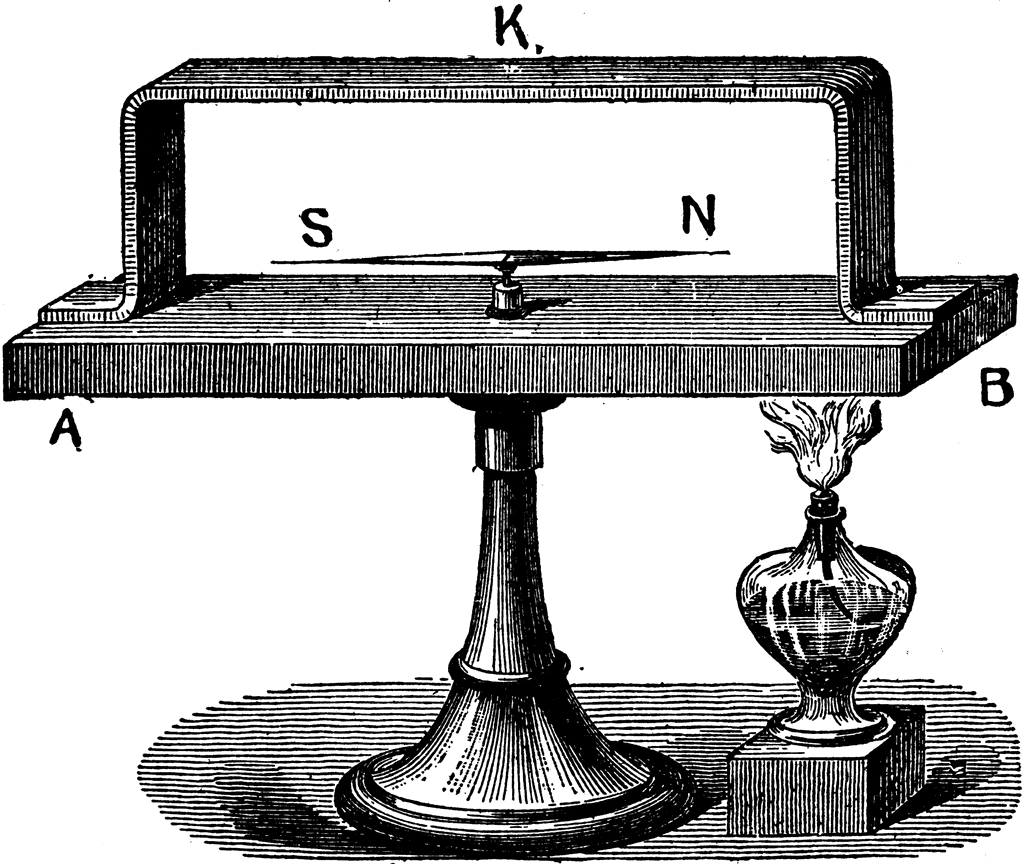
\includegraphics[width=0.5\textwidth]{seebeck-experiment-black.png}
	\caption{Thomas Seebeck's original thermoelectricity experiment
	diagram \cite{seebeck-original}. A compass needle lies on top of
	one metal, underneath a bridge of a different metal (K), connected
	by two junctions and heated at one of these junctions.}
	\label{seebeck-experiment}
\end{figure}

\begin{figure}
	\centering
	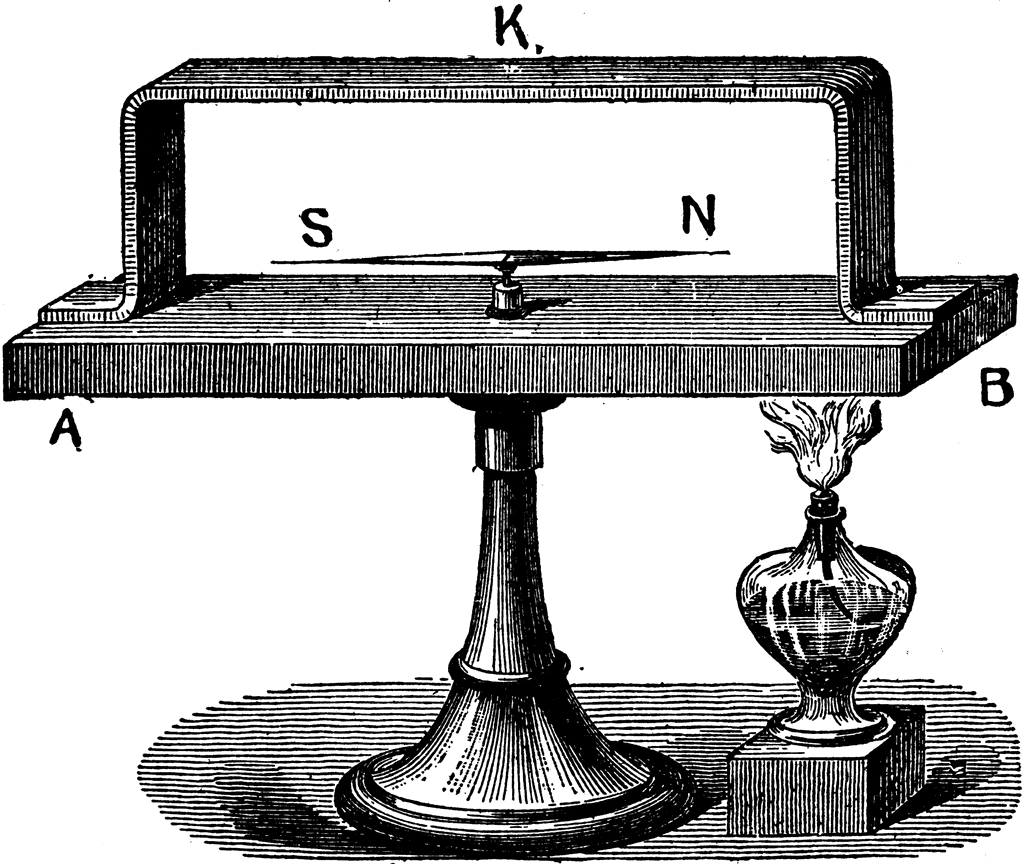
\includegraphics[width=0.5\textwidth]{seebeck-experiment-black.png}
	\caption{Thomas Seebeck's original thermoelectricity experiment
	diagram \cite{seebeck-original}. A compass needle lies on top of
	one metal, underneath a bridge of a different metal (K), connected
	by two junctions and heated at one of these junctions.}
	\label{seebeck-experiment}
\end{figure}

\subsection{Statistical Mechanics}
Using the kinetic theory, with relevant assumptions defined in \secref{project-discussion}, the charge density
$\vec{J}$ of an arbitrary charge carrier can be described
microscopically \cite{kittel}:

\begin{equation}
\label{charge-density}
	\vec{J} = \frac{nq^2\vec{E} \tau}{m}
\end{equation}
where $n$ is free charge carrier density, $q$ is the charge of the
carrier, $\vec{E}$ is the electric field accelerating the
carrier, $\tau$ is the mean time between carrier collisions and $m$ is
carrier mass.

Applying this to solid-state electrical conductivity $\sigma = \frac{ne^2
\tau}{m^*}$ it can be shown that \cite{ziman}:

\begin{equation}
\label{micro-elec}
	\sigma = \frac{e^2}{m^*} \sum_{\mathrm{spin}} \sum_{\vec{k}}
	n(\vec{k}) \tau(\vec{k})
\end{equation}
where $e$ is electron charge, $m^*$ is the electron effective mass, $\mathrm{spin}$ refers to
electron spin and $\vec{k}$ is the electron wavevector over the
Brillouin zone. These new concepts are all derived from the nearly free electron
model, as described in Kittel \cite{kittel}.

The Boltzmann transport equation ``describes the statistical behaviour
of a thermodynamic system not in thermodynamic equilibrium"
\cite{wiki-boltz} and its general definition is:

\begin{equation}
\label{boltz-trans}
	\frac{\partial f}{\partial t} = \left(\frac{\partial f}{\partial
	t}\right)_\mathrm{force} + \left(\frac{\partial f}{\partial t}\right)_\mathrm{diff}+ \left(\frac{\partial f}{\partial t}\right)_\mathrm{coll}
\end{equation}
where $\frac{\partial f}{\partial t}$ is time dependence of a system
of particles $f$, the ``force" term represents external forces on the
particles, the ``diff" term is the diffusion of particles through the
system and the ``coll" term represents forces acting between particles
in collisions.

A phonon is the quantisation of vibrational motion of a lattice of
atoms at a single frequency, known as a normal mode \cite{kittel}. These phonons are
quasiparticles, free to move around the lattice and they are
distributed according to the Bose-Einstein distribution \cite{kittel}:

\begin{equation}
\label{bose-einstein}
	 \bar{n} = \frac{1}{e^{(\hbar \omega) / k T} - 1}
\end{equation}
where $\bar{n}$ is the probability of a phonon existing with energy
$\hbar \omega$.\\
Electrons can be modelled as quasiparticles in a similar way, with a
wavevector and effective mass as in equation \eqref{micro-elec},
leading to the Fermi-Dirac distribution \cite{kittel}:

\begin{equation}
\label{fermi-dirac}
	 \bar{f} = \frac{1}{e^{(E - E_f) / k T} + 1}
\end{equation}
where $\bar{f}$ is the probability of an electron existing with energy
$E$ and $E_f$ is the Fermi level.\\
In the presence of an external fields, phonon and electron
distributions (\eqref{bose-einstein} \& \eqref{fermi-dirac}) both
satisfy the Boltzmann transport equation \eqref{boltz-trans} with
\cite{ziman}:

\begin{equation}
\label{boltz-specific}
	\frac{df}{dt}\bigg|_{field} + \frac{df}{dt}\bigg|_{collisions} = 0
\end{equation}
where function $f$ is $f = \bar{n}$ or $f = \bar{f}$, the Bose-Einstein
and Fermi-Dirac distribution functions.

\subsection{Nanocomposites}

Composite materials are combinations of two or more materials, forming a new structure with significantly different physical or chemical properties than its constituent parts. In a similar way, nanocomposites are the structuring of multiple materials, but at the nanoscale. As our nanocomposites are at a comparable size to the crystal lattices of their constituent materials, we can view
nanocomposites as artificial defects in a larger crystal lattice. A
simple example of a 2D nanocomposite, a copper-graphene superlattice,
is pictured in \figref{superlattice}. Examining one layer of the
superlattice, the material in bulk form would be a 3D crystal structure,
but by constraining the layer thickness we have introduced a boundary
defect. The periodic array of these boundary defects forms a new 3D
artificial crystal, which we define as a superlattice, a nanocomposite.

\begin{figure}
	\centering
	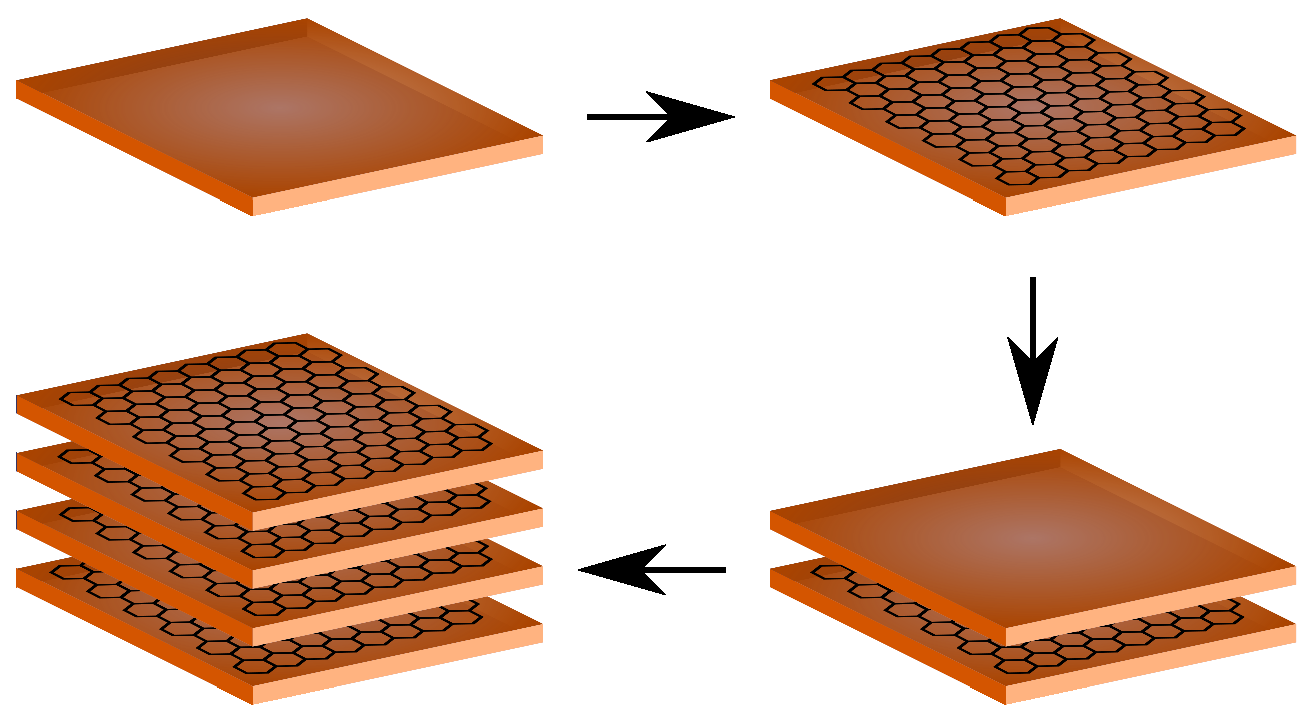
\includegraphics[width=0.5\textwidth]{graphene-superlattice.eps}
	\caption{Superlattice of graphene and copper. Alternate layers of
	nanoscale copper and graphene are sandwiched together.}
\end{figure}

\section{Specfic Theory}
% Details of exactly what you've done
% Tell a story, keep it concise, only explain what you need to
\subsection{Assumptions}
For our project we will be using the phonon and nearly free electron models, which
bring with them a multitude of assumptions. For the phonon model, our
main assumption is that our system consists of at least 50 atomic oscillators
\cite{kittel}; this means we are limited to a $50\r{A} = 5
\mathrm{nm}$ fabrication size. Current fabrication methods are at best
25nm \cite{minnich-review}, so our 50 oscillator assumption is well met.
For both the phonon and the nearly free electron model, we assume an ideal gas,
i.e., particles do not interact with each other and can move freely
around the lattice, affected only by lattice perturbations. This is
known to be a good assumption for the low temperatures found in solid-state physics
\cite{kittel}.\\
Based on this limited initial analysis, we believe these assumptions
should be valid. If it transpires that these assumptions cannot be met, we will seek alternative models.\\

\subsection{Thermoelectric Efficiency}
The thermoelectric efficiency is best expressed in the dimensionless
parameter $ZT$ with thermal efficiency $\eta$ which is a function of $(ZT, T_h,
T_c)$, where $Z$ is the figure of merit, $T = \frac{1}{2}(T_h +
T_c)$, $T_h$ is the temperature at the hot junction and $T_c$ is the
temperature at the cold junction. $ZT$:
\begin{equation}
\label{zt}
	ZT = \frac{S^2 \sigma T}{\kappa_e + \kappa_{ph}}
\end{equation}
where $S$ is the Seebeck coefficient from equation \eqref{seebeck-emf}
\& \eqref{current-density}, $\sigma$ is electrical conductivity,
$\kappa_e$ and $\kappa_{ph}$ are the thermal conductivity due to
electrons and phonons respectively. This is derived in D. M. Rowe's Modern
Thermoelectrics \cite{modern-thermoelectrics}.\\
Important points to note about $ZT$ are that it is proportional to thermal efficiency $\eta$, is increased by a reduction in thermal conductivity and it depends on the square of the Seebeck coefficient. Figure \figref{zt-dope} demonstrates the comprimise between the variables in equation \eqref{zt}. $ZT$ values of current generation thermoelectric materials have been plotted in figure \figref{zt-plot}.

\begin{figure}
	\centering
	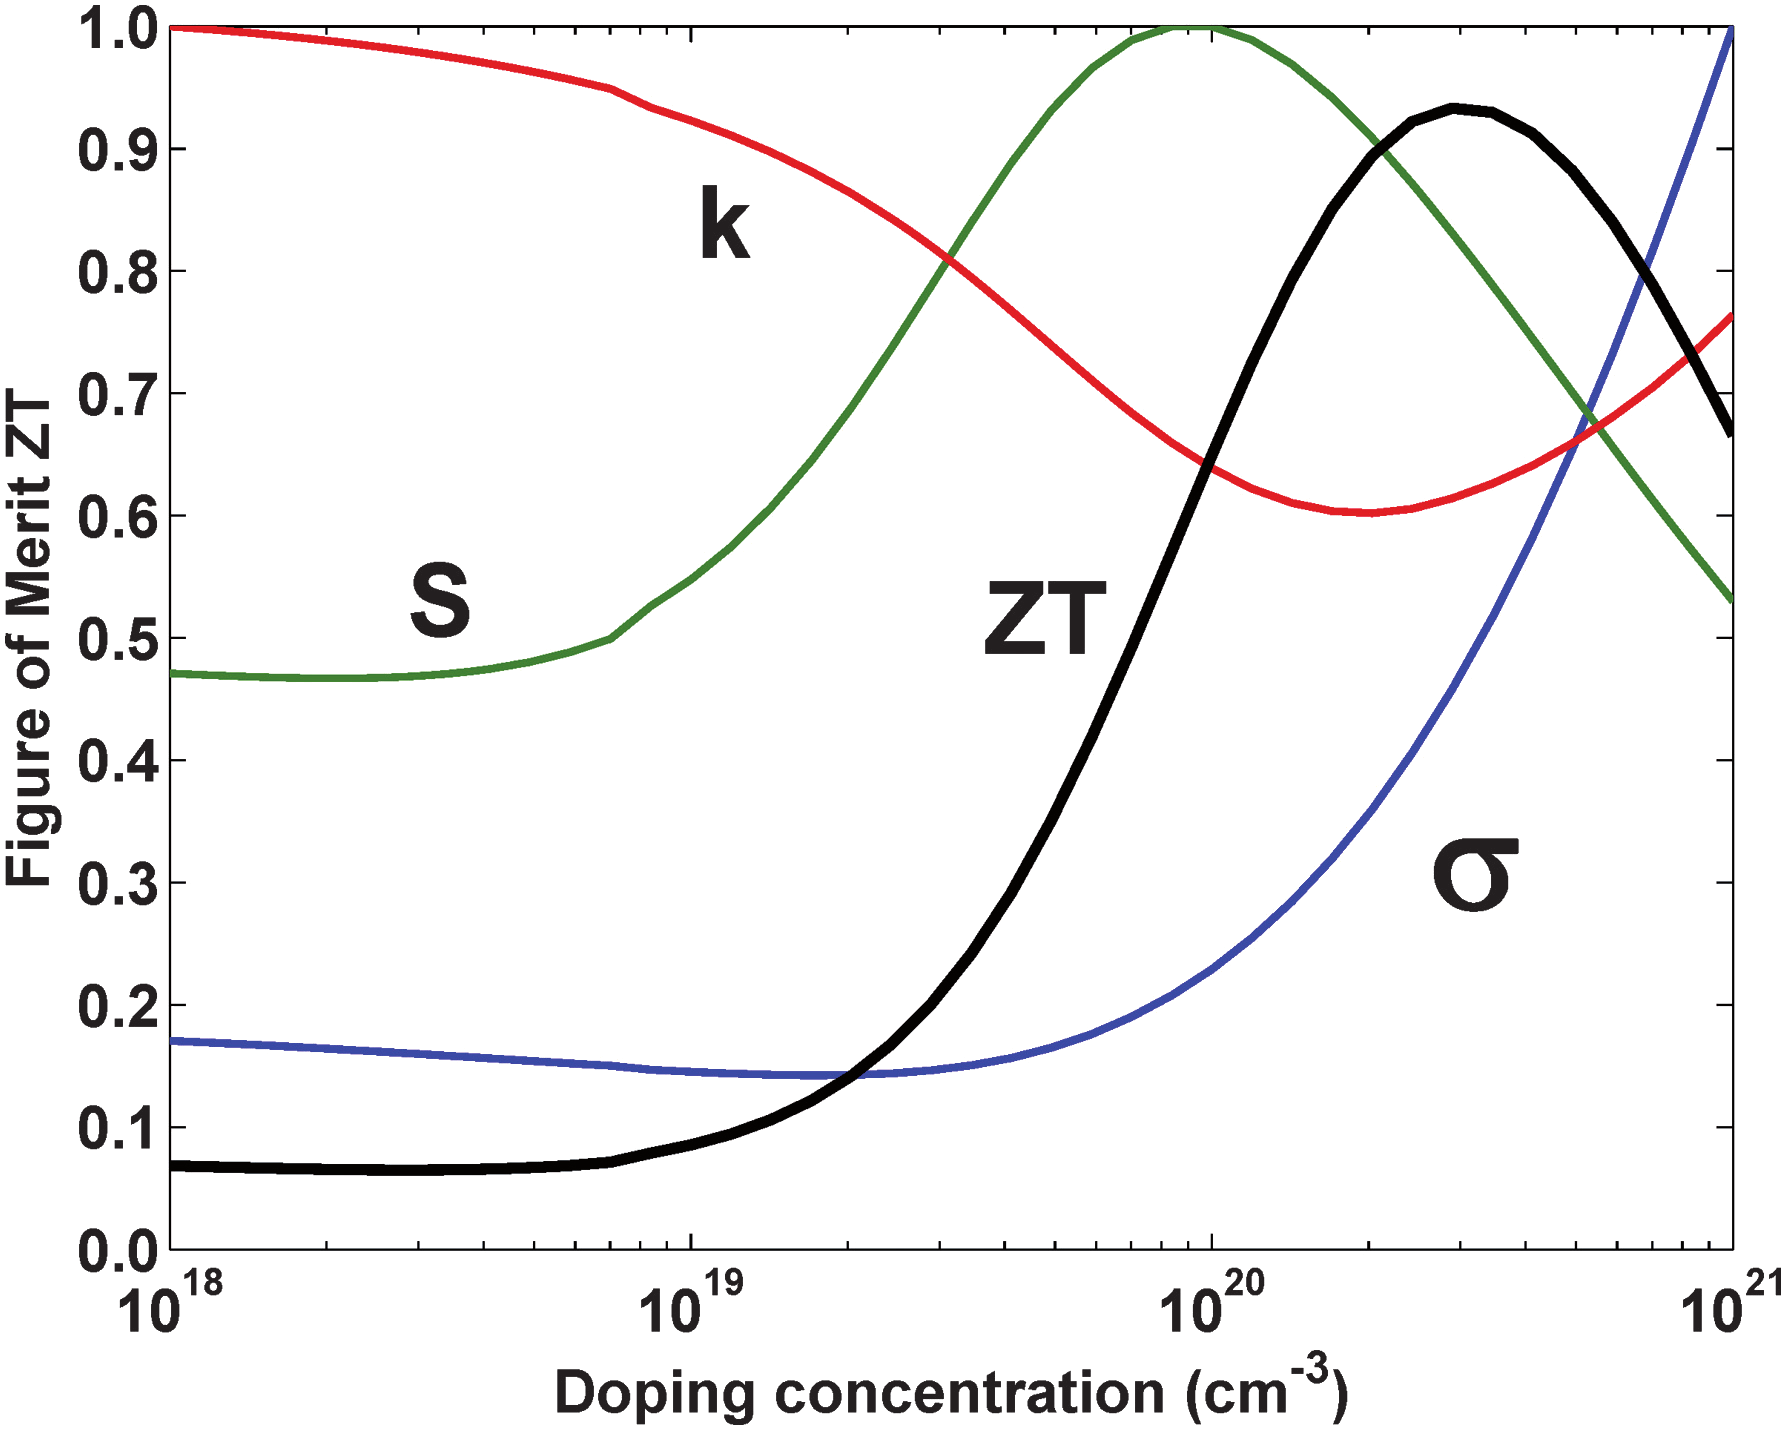
\includegraphics[width=0.5\textwidth]{zt-dope-plot.png}
	\caption{Graph of doping concentration (electron density) against $ZT$.  Insulators are seen up to $10^{19}$ with semi-conductors occupying the rest of the range. A compromise between variables $\sigma, \kappa, S^2$, results in heavily doped semi-conductors at the $ZT$ peak \cite{minnich-review}.}
	\label{zt-dope}
\end{figure}

\begin{figure}
	\centering
	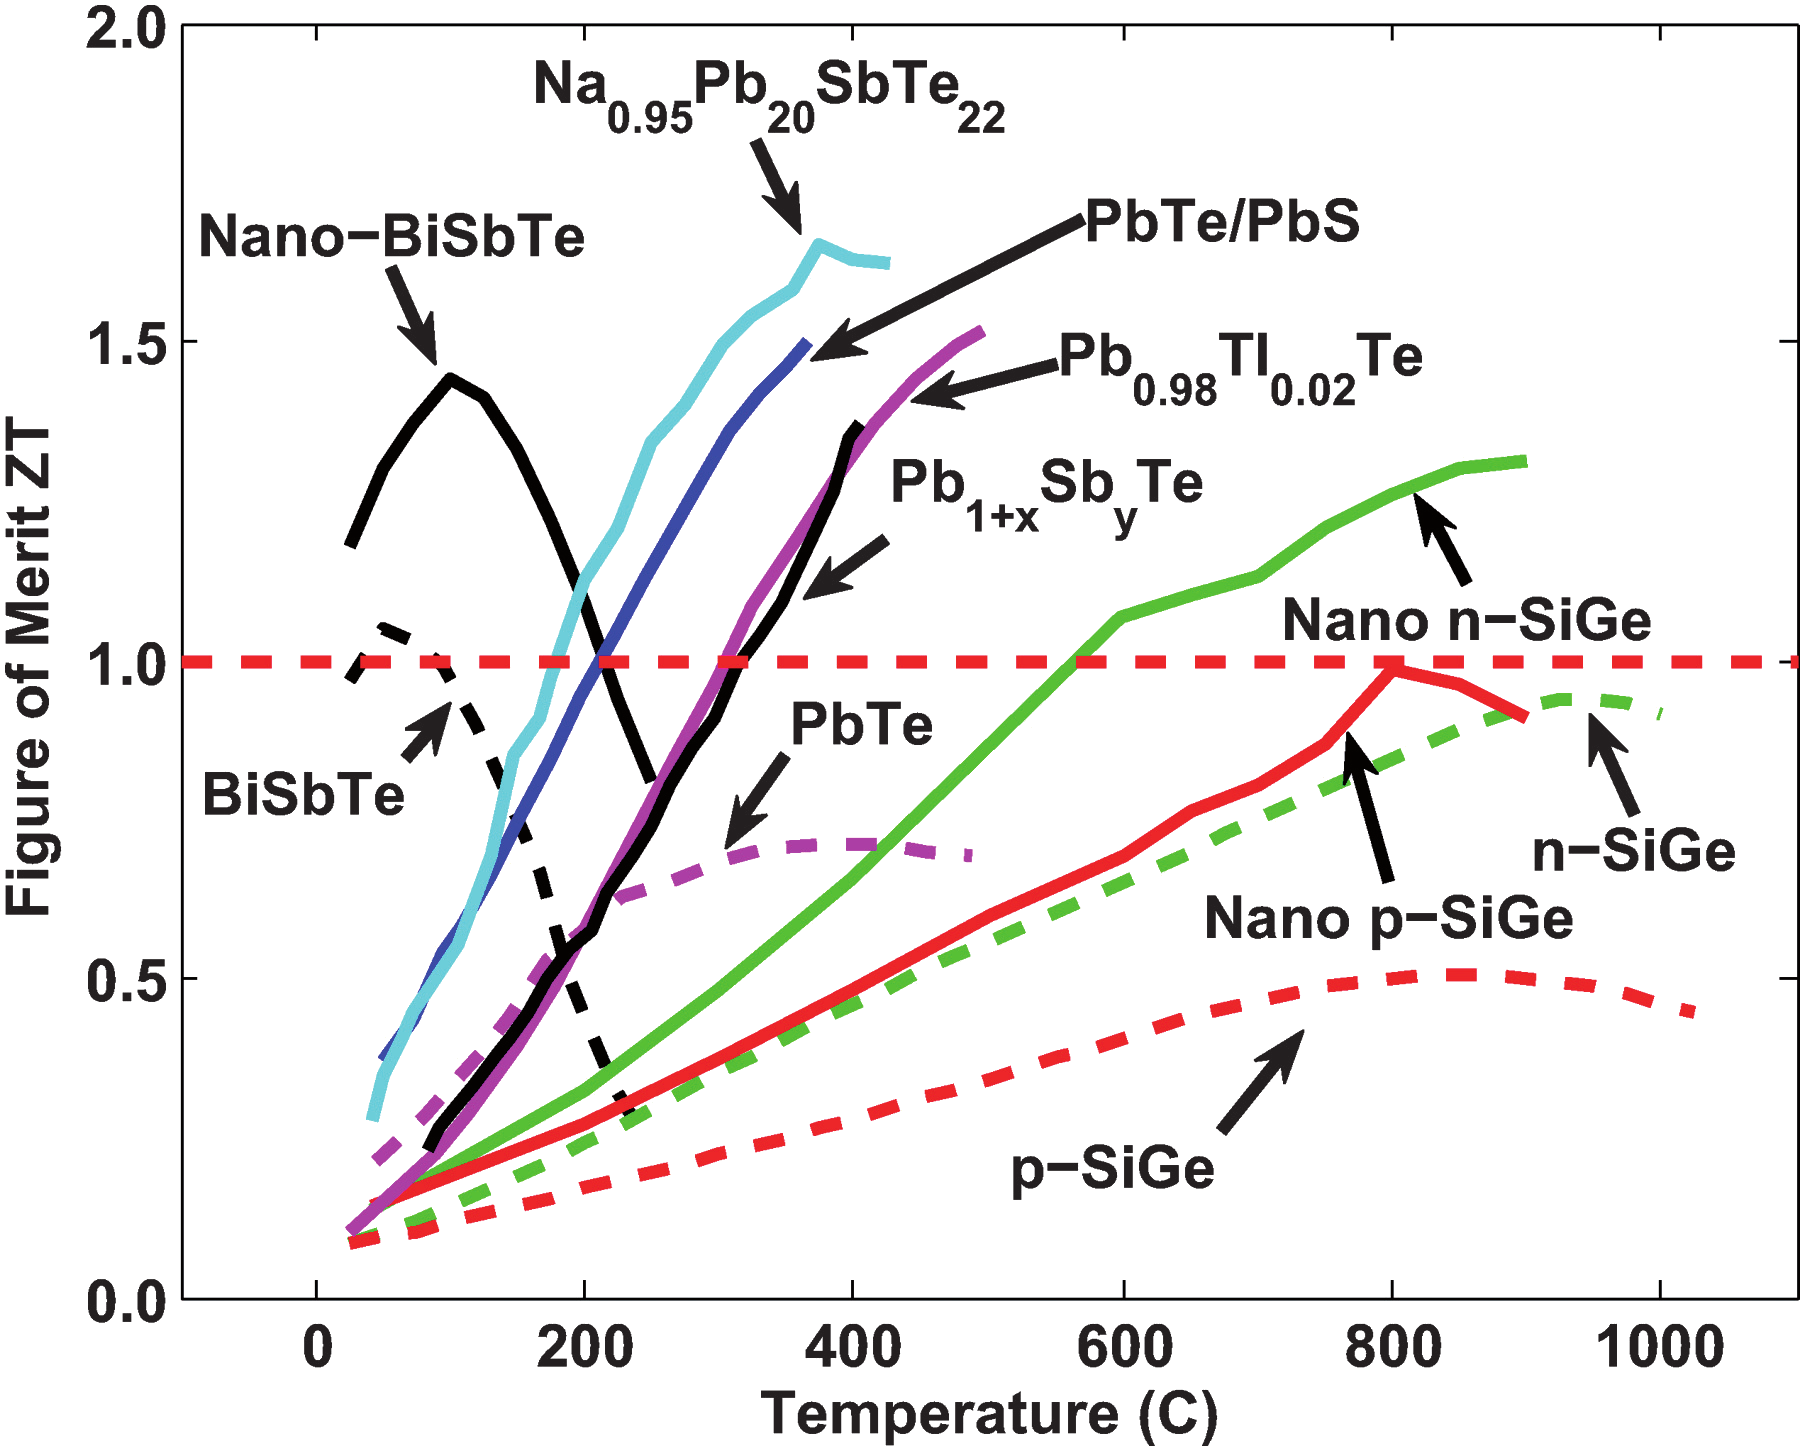
\includegraphics[width=0.5\textwidth]{zt-temp-plot.png}
	\caption{Graph of thermoelectric figure of merit $ZT$ against
	temperature. The dashed line represents bulk thermoelectric materials, above the dashed line shows current generation nanocomposites \cite{minnich-review}.}
	\label{zt-plot}
\end{figure}

\subsection{Phonon Glass Electron Crystal}
A core concept for for our project is the idea of \ac{PGEC} first proposed by G. A. Slack \cite{crc-handbook}. Slack proposes that developing a material with the properties of both phonon scattering glasses and electron transmissive crystals, will achieve the desired $ZT > 3$. It is thought that the low dimensional systems of nanocomposites introduce the short range disorder of crystal structures common to glasses, yet they maintain the long range order common to electron crystals common \cite{crc-handbook}. Some key questions for our project are; How can we achieve \ac{PGEC}? What are its constraints? How effective is it at increasing $ZT$?

\section{Project Aims}
Thermoelectric theory provides a good basis from which we can
understand solid-state physics. Using phonon and nearly free electron models together with
the Boltzmann transport equation \eqref{boltz-trans} we aim to develop
a \ac{PGEC} inspired mechanism through which $ZT$ can be increased. If such a mechanism is found we will design novel structures and model them computationally. In pursuit of this aim, it is
likely that we utilise nanocomposite material design for the
introduction of multiple boundary defects.

\url{https://github.com/kahlos/thermoelectrics}

\bibliographystyle{IEEEtran}
\begin{thebibliography}{5}
\bibitem{crc-handbook}
G. A. Slack, \emph{CRC Handbook of Thermoelectrics}. Ed D. M. Rowe, CRC Press, 1995
\bibitem{minnich-review}
A. J. Minnich et al. \emph{Bulk nanostructured thermoelectric
materials: current research and future prospects}. Energy Environ.
Sci., 2009, 2, 466-479. DOI: 10.1039/B822664B
\bibitem{engine-efficiency}
L. M. Baglione, \emph{Development of System Analysis Methodologies and Tools for Modeling and Optimizing Vehicle System Efficiency} University of Michigan, 2009, . pp. 52�54.
\bibitem{seebeck-original}
\url{etc.usf.edu/clipart/35600/35659/seebeck_35659_lg.gif} 24 November
2013
\bibitem{bos-review}
J. W. Bos, \emph{Thermoelectric materials: efficiencies found in
nanocomposites}. Education in Chemistry, March 2012. Available
from:
\url{http://www.rsc.org/images/Thermoelectric-materials_tcm18-214041.pdf} 24 November 2013
\bibitem{auparay}
N. Auparay, \emph{Room Temperature Seebeck Coefficient Measurement
of Metals and Semiconductors}. Available
from:
\url{http://www.physics.oregonstate.edu/~tate/TateLabWiki/lib/exe/fetch.php?media=theses:auparay_bs_2013.pdf} 20 November 2013
\bibitem{ziman}
%p270-275, section 7.5 & 7,6
J. M. Ziman, \emph{Electrons and Phonons: The Theory of Transport
Phenomena in Solids}. 1960, ISBN: 978-0-19-850779-6
\bibitem{kittel}
C. Kittel, \emph{Introduction to Solid State Physics, 8th ed}. November 2004, ISBN: 978-0471415268
\bibitem{wiki-boltz}
\url{http://en.wikipedia.org/wiki/Boltzmann_equation} 18 November 2013
\bibitem{modern-thermoelectrics}
D. M. Rowe, \emph{Modern Thermoelectrics}. Reston Pub Co, September
1983. ISBN: 978-0835945936
\end{thebibliography}

\end{document}

%shifted out of document probably not going to use
\newpage
\appendix


\section{Further Questions and Thoughts}

\section{List of Assumptions}

\section{Further Reading}

\section{Tools and Software}

\section{Physical Data}

\section{Program Code}
%abbrivations list%
\acresetall
\ac{PGEC} - Exhibiting the properties of phonon scattering glasses and
electron transmissive crystals
\ac{SSP} - The study of rigid matter (solids)

\section{Open Questions}
These questions are ideas that I have posed thus far in the project.
They are included as an interest to the reader, perhaps indicating
area of further study

\begin{itemize}
  \item Can acoustic stimulation of a material cause additional phonon
  collisions? Is a $kappa_{ph}$ reduction obtainable?
\end{itemize}